% 第11章第9节：线性作用的误差放大与条件数（输入扰动与误差尺度，固定输入处的条件数，矩阵条件数与方向差异）。

\section{线性作用的误差放大与条件数}
\label{sec:ls-perturbation}
\label{sec:linear-algebra-stability}
\label{sec:matrix-analysis-conditioning-perturbation}

前面几节为线性作用找到了便于理解的表示，并用它们解决了几个最优选择问题。从本节起转向另一类问题：数据不精确时，由它算出的结论还有多可靠。固定矩阵$\bm A$，理想输入是$\bm x$，实际只能测到$\bm x+\bm h$，输出$\bm A(\bm x+\bm h)$与理想输出$\bm A\bm x$相差多少？允许范围内的输入增量$\bm h$称为\term{扰动}（perturbation）。

本节分三步回答。先确定怎样度量输入与输出的误差，比较绝对误差与相对误差；再固定输入$\bm x$，对扰动方向取最坏值，得到绝对条件数与相对条件数；最后对输入方向也取最坏值，得到只依赖矩阵的条件数，并用奇异值说明它比较的是最强与最弱作用的差异。除特别说明外，向量使用欧氏范数，矩阵使用相应的谱范数。本节讨论的是输入数据的误差怎样传播，矩阵本身和计算过程都视为精确；算法在计算中引入的误差由第~\ref{chap:linear-equations-and-optimization}章另行讨论。

\subsection{输入扰动与误差尺度}
\label{sec:ls-input-error-scales}

设理想输出为$\bm y=\bm A\bm x$，其中$\bm A\in\mathbb R^{m\times n}$固定。实际输入为$\bm x+\bm h$时，输出的精确变化是
\[
 \Delta\bm y=\bm A(\bm x+\bm h)-\bm A\bm x=\bm A\bm h .
\]
这一等式只用到矩阵乘法的分配律，对任意大小的$\bm h$都成立，不需要微分，也不要求扰动很小。实际中通常不知道$\bm h$本身，只知道误差的预算：给定$\eta\geq0$，已知$\lVert\bm h\rVert_2\leq\eta$。本节要回答两个问题：输出误差$\lVert\bm A\bm h\rVert_2$有什么可靠的上界；哪些扰动方向会达到或接近这个上界。

回答之前先约定误差的读法。输入与输出的\term{绝对误差}（absolute error）分别是增量的长度$\lVert\bm h\rVert_2$与$\lVert\bm A\bm h\rVert_2$。当量本身有尺度时，更常用增量占原量的比例：在$\bm x\neq\bm0$且$\bm A\bm x\neq\bm0$时，输入与输出的\term{相对误差}（relative error）分别是
\[
 \frac{\lVert\bm h\rVert_2}{\lVert\bm x\rVert_2},\qquad
 \frac{\lVert\bm A\bm h\rVert_2}{\lVert\bm A\bm x\rVert_2}.
\]
把输入和扰动同乘一个非零常数，输出和输出增量也同乘这个常数，两端的相对误差都不变，所以相对误差反映的是变化占原有量的比例。但参照量为零时它没有定义，例如$\bm A\bm x=\bm0$时只能报告输出的绝对误差；参照量接近零时，很小的绝对变化也会造成很大的相对误差，这时应同时报告绝对误差。选用哪种范数、两端各按绝对还是相对尺度比较，都属于问题本身的规定；规定不同，得到的敏感程度一般也不同。

即使规定相同，同一个矩阵在不同的基点和扰动方向上，相对误差的放大也可以很不一样。
\begin{example}[对角矩阵的两种基点]
\label{ex:ls-diagonal-relative-error-basepoints}
取$\bm A=\operatorname{diag}(1,s)$，$0<s<1$，误差预算$\eta>0$。

先取$\bm x=\bm e_2$、$\bm h=\eta\bm e_1$。此时$\bm A\bm x=s\bm e_2$，$\bm A\bm h=\eta\bm e_1$，输入与输出的绝对误差都是$\eta$。输入相对误差为$\eta/1=\eta$，输出相对误差却是$\eta/s$，放大了$1/s$倍。原因是理想输出被压缩到原来的$s$倍，分母变小了，而扰动所在的$\bm e_1$方向没有被压缩。

保持同一矩阵，改取$\bm x=\bm e_1$、$\bm h=\eta\bm e_2$。此时$\bm A\bm x=\bm e_1$，$\bm A\bm h=s\eta\bm e_2$，输入相对误差为$\eta$，输出相对误差为$s\eta$，两者之比为$s<1$，误差反而被缩小。
\end{example}
两种取法用的是同一个矩阵，相对误差之比却从$1/s$变成$s$。所以谈论矩阵对相对误差的放大时，必须说明基点和扰动方向，或者对它们取最坏情形；下一小节按后一种方式定义条件数。

相对误差的放大也不只来自矩阵对不同方向压缩程度的差别。理想输出本身很小时，即使绝对误差没有被放大，相对误差也会被放大，最常见的情形是两个相近的数相减。
\begin{example}[加法中的抵消]
\label{ex:ls-cancellation-relative-error}
取行矩阵$\bm A=\begin{bmatrix}1&1\end{bmatrix}$，它把输入的两个分量相加。理想输入为$\bm x=(1.0001,-1.0000)^\top$，两个分量各带至多$5\times10^{-5}$的绝对误差，即扰动$\bm h=(h_1,h_2)^\top$满足$|h_1|,|h_2|\leq5\times10^{-5}$。理想输出为$\bm A\bm x=10^{-4}$，输出的精确增量为$\bm A\bm h=h_1+h_2$。由三角不等式，
\[
 |h_1+h_2|\leq|h_1|+|h_2|\leq10^{-4},
\]
取$h_1=h_2=5\times10^{-5}$时等号成立，所以输出的相对误差可达
\[
 \frac{10^{-4}}{10^{-4}}=1 .
\]
另一方面，$\lVert\bm h\rVert_2\leq\sqrt2\times5\times10^{-5}$，$\lVert\bm x\rVert_2\approx\sqrt2$，输入的相对误差至多约为$5\times10^{-5}$。相对误差被放大约$2\times10^4$倍。
\end{example}
这里只用了精确增量与三角不等式。放大也不是算法造成的舍入误差：即使加法精确执行，输入误差本身就使输出的相对误差这样放大，这是问题在相对尺度下的敏感性。

\subsection{固定输入处的条件数}
\label{sec:ls-perturbation-conditioning}

上一小节的例子都只看了个别扰动方向。误差预算只限制$\lVert\bm h\rVert_2$，不限制方向，所以可靠的误差界必须对所有方向成立，由最坏的方向决定。先看绝对误差。

对非零扰动$\bm h$，比较输出与输入的绝对误差之比$\lVert\bm A\bm h\rVert_2/\lVert\bm h\rVert_2$。把$\bm h$换成$c\bm h$（$c\neq0$）时，分子与分母同乘$|c|$，所以这个比值只依赖扰动的方向，与扰动的大小无关，也与基点$\bm x$无关。它在全部非零扰动上的上确界就是第~\ref{sec:ls-matrix-norms}节的诱导范数$\lVert\bm A\rVert_2$，称为线性作用$\bm x\mapsto\bm A\bm x$的\term{绝对条件数}（absolute condition number）。由第~\ref{sec:ls-svd}节的式~\eqref{eq:matrix-analysis-spectral-norm}，它等于最大奇异值$\sigma_{\max}(\bm A)$。下面把这一事实写成可以直接使用的误差界，并说明它不能再改进。

\begin{theorem}[线性作用的绝对误差界]
\label{thm:ls-absolute-error-bound}
设$\bm A\in\mathbb R^{m\times n}$的最大奇异值为$\sigma_{\max}(\bm A)$，对应的单位右奇异向量为$\bm v_1$。对任意$\bm h\in\mathbb R^n$，
\[
 \lVert\bm A\bm h\rVert_2\leq\sigma_{\max}(\bm A)\lVert\bm h\rVert_2 ,
\]
且$\bm h=\eta\bm v_1$时等号成立。因此在误差预算$\lVert\bm h\rVert_2\leq\eta$下，$\sigma_{\max}(\bm A)\eta$是输出绝对误差的上界，并且不存在更小的常数$c$使$\lVert\bm A\bm h\rVert_2\leq c\eta$对所有这样的$\bm h$成立。
\end{theorem}
\begin{proof}
把$\bm h$按右奇异向量展开为$\bm h=\sum_ic_i\bm v_i$，则$\lVert\bm A\bm h\rVert_2^2=\sum_i\sigma_i^2c_i^2\leq\sigma_{\max}^2\sum_ic_i^2=\sigma_{\max}^2\lVert\bm h\rVert_2^2$，这就是不等式。取$\bm h=\eta\bm v_1$时，$\bm A\bm h=\eta\sigma_{\max}\bm u_1$，长度恰为$\sigma_{\max}\eta$。若$c<\sigma_{\max}$且$\eta>0$，这个扰动满足预算却有$\lVert\bm A\bm h\rVert_2>c\eta$；$\eta=0$时结论平凡。
\end{proof}

再看相对误差。固定基点$\bm x$，两端都改用相对尺度，再对扰动方向取最坏情形。
\begin{definition}[线性作用的相对条件数]
\label{def:ls-relative-condition-number}
设$\bm x\neq\bm0$且$\bm A\bm x\neq\bm0$。称
\[
 \kappa_{\mathrm{rel}}(\bm A;\bm x)
 =\sup_{\bm h\neq\bm0}
 \frac{\lVert\bm A\bm h\rVert_2/\lVert\bm A\bm x\rVert_2}
      {\lVert\bm h\rVert_2/\lVert\bm x\rVert_2}
\]
为线性作用$\bm x\mapsto\bm A\bm x$在$\bm x$处的\term{相对条件数}（relative condition number）。
\end{definition}
这个上确界可以直接算出，并给出对任意扰动成立的相对误差界。
\begin{theorem}[相对条件数与相对误差界]
\label{thm:ls-relative-condition-number}
在定义~\ref{def:ls-relative-condition-number}的条件下，
\[
 \kappa_{\mathrm{rel}}(\bm A;\bm x)=\frac{\lVert\bm A\rVert_2\lVert\bm x\rVert_2}{\lVert\bm A\bm x\rVert_2},
\]
并且对任意$\bm h\in\mathbb R^n$，
\begin{equation}
 \frac{\lVert\bm A\bm h\rVert_2}{\lVert\bm A\bm x\rVert_2}
 \leq\kappa_{\mathrm{rel}}(\bm A;\bm x)\,\frac{\lVert\bm h\rVert_2}{\lVert\bm x\rVert_2},
 \label{eq:matrix-analysis-condition-number-bound}
\end{equation}
扰动沿最大右奇异方向$\bm h=c\bm v_1$（$c\neq0$）时等号成立。
\end{theorem}
\begin{proof}
对$\bm h\neq\bm0$，定义中的比值可以写成
\[
 \frac{\lVert\bm x\rVert_2}{\lVert\bm A\bm x\rVert_2}\cdot
 \frac{\lVert\bm A\bm h\rVert_2}{\lVert\bm h\rVert_2}.
\]
第一个因子与$\bm h$无关；由定理~\ref{thm:ls-absolute-error-bound}，第二个因子的上确界是$\lVert\bm A\rVert_2=\sigma_{\max}(\bm A)$，并在$\bm h=c\bm v_1$时取到。这就得到$\kappa_{\mathrm{rel}}$的表达式和等号条件。不等式~\eqref{eq:matrix-analysis-condition-number-bound}在$\bm h\neq\bm0$时是上确界定义的改写，$\bm h=\bm0$时两端都为零。
\end{proof}
相对条件数描述的是：基点固定在$\bm x$，扰动方向任意时，相对误差最多放大多少倍。回到示例~\ref{ex:ls-diagonal-relative-error-basepoints}：$\lVert\bm A\rVert_2=1$，在$\bm x=\bm e_2$处$\kappa_{\mathrm{rel}}=1\cdot1/s=1/s$，示例中的扰动$\eta\bm e_1$恰沿最大右奇异方向，达到了这个值；在$\bm x=\bm e_1$处$\kappa_{\mathrm{rel}}=1$。沿某一个具体方向实际观察到的比值可以更小，例如在$\bm x=\bm e_2$处取$\bm h=\eta\bm e_2$，输出相对误差为$s\eta/s=\eta$，比值只有$1$。

上面的两个上确界都取遍全部非零的有限扰动，而不是先让扰动趋于零。这样做可行，是因为线性作用的误差比与扰动的大小无关，只依赖方向；所以定理中的误差界对任意大小的扰动都成立。一般非线性映射$F$的输出增量$F(\bm z+\bm h)-F(\bm z)$不再与$\bm h$成比例，误差比会随扰动半径变化。那时要先在半径为$\delta$的扰动中取最坏值，再令$\delta$缩小，用第~\ref{sec:multivariable-limits-continuity}节的极限定义局部条件数，并在可微条件下把它与微分的范数联系起来，这些在第~\ref{sec:multivariable-local-condition-number}节建立。本节只讨论线性作用，不用一般映射的定义代替这里的直接推导。

\subsection{矩阵条件数与方向差异}
\label{sec:ls-matrix-condition-number}

相对条件数随基点变化：基点落在被压缩的方向上时，$\lVert\bm A\bm x\rVert_2$小，相对条件数大。若事先不知道输入落在哪里，就要对基点也取最坏值。对可逆方阵，这个最坏值只依赖矩阵本身。

\begin{definition}[可逆矩阵的条件数]
\label{def:matrix-analysis-condition-number}
对同一向量范数诱导的矩阵范数，可逆方阵$\bm A$的\term{条件数}（condition number）为
\begin{equation}
 \kappa(\bm A)=\lVert\bm A\rVert\,\lVert\bm A^{-1}\rVert .
 \label{eq:matrix-analysis-condition-number}
\end{equation}
欧氏范数下记为$\kappa_2(\bm A)$。
\end{definition}

下面的定理说明，这个数正是相对条件数对全部基点的最坏值，并由奇异值读出。
\begin{theorem}[条件数是相对条件数的最坏值]
\label{thm:matrix-analysis-condition-number-bound}
设$\bm A\in\mathbb R^{n\times n}$可逆，奇异值为$\sigma_{\max}=\sigma_1\geq\cdots\geq\sigma_n=\sigma_{\min}>0$，对应的单位右奇异向量为$\bm v_1,\ldots,\bm v_n$。则
\begin{enumerate}
 \item 对全部非零基点取最坏值，
 \begin{equation}
  \sup_{\bm x\neq\bm0}\kappa_{\mathrm{rel}}(\bm A;\bm x)
  =\kappa_2(\bm A)
  =\frac{\sigma_{\max}(\bm A)}{\sigma_{\min}(\bm A)},
  \label{eq:matrix-analysis-spectral-condition-number}
 \end{equation}
 且上确界在$\bm x=\bm v_n$处取到；
 \item 对任意$\bm x\neq\bm0$与任意$\bm h$，
 \[
  \frac{\lVert\bm A\bm h\rVert_2}{\lVert\bm A\bm x\rVert_2}
  \leq\kappa_2(\bm A)\,\frac{\lVert\bm h\rVert_2}{\lVert\bm x\rVert_2},
 \]
 当$\bm x=\bm v_n$、$\bm h=c\bm v_1$（$c\neq0$）时等号成立；
 \item 特别地，对可逆方程$\bm A\bm x=\bm b$（$\bm b\neq\bm0$），右端改为$\bm b+\Delta\bm b$时，解的增量$\Delta\bm x$对任意大小的$\Delta\bm b$都满足
 \[
  \frac{\lVert\Delta\bm x\rVert_2}{\lVert\bm x\rVert_2}
  \leq\kappa_2(\bm A)\,\frac{\lVert\Delta\bm b\rVert_2}{\lVert\bm b\rVert_2}.
 \]
\end{enumerate}
\end{theorem}
\begin{proof}
先证第1条。把$\bm x$按右奇异向量展开为$\bm x=\sum_ic_i\bm v_i$，则
\[
 \lVert\bm A\bm x\rVert_2^2=\sum_i\sigma_i^2c_i^2\geq\sigma_n^2\sum_ic_i^2=\sigma_n^2\lVert\bm x\rVert_2^2 ,
\]
等号在$\bm x=\bm v_n$时成立。由定理~\ref{thm:ls-relative-condition-number}，
\[
 \kappa_{\mathrm{rel}}(\bm A;\bm x)=\frac{\sigma_1\lVert\bm x\rVert_2}{\lVert\bm A\bm x\rVert_2}\leq\frac{\sigma_1}{\sigma_n},
\]
在$\bm x=\bm v_n$时取等号，所以上确界等于$\sigma_1/\sigma_n$且取到。又由第~\ref{sec:ls-svd}节，$\lVert\bm A\rVert_2=\sigma_1$、$\lVert\bm A^{-1}\rVert_2=1/\sigma_n$，故$\sigma_1/\sigma_n=\kappa_2(\bm A)$。

第2条：$\bm A$可逆且$\bm x\neq\bm0$，所以$\bm A\bm x\neq\bm0$，可以使用式~\eqref{eq:matrix-analysis-condition-number-bound}，再用第1条把$\kappa_{\mathrm{rel}}(\bm A;\bm x)$放大为$\kappa_2(\bm A)$。$\bm x=\bm v_n$时第一步放大取等号；$\bm h=c\bm v_1$时式~\eqref{eq:matrix-analysis-condition-number-bound}取等号。

第3条：由$\bm A(\bm x+\Delta\bm x)=\bm b+\Delta\bm b$减去$\bm A\bm x=\bm b$，得$\Delta\bm x=\bm A^{-1}\Delta\bm b$。这是线性作用$\bm A^{-1}$在基点$\bm b$处对扰动$\Delta\bm b$的输出增量，理想输出为$\bm A^{-1}\bm b=\bm x\neq\bm0$。把第2条用于$\bm A^{-1}$，并注意$\bm A^{-1}$的奇异值是$1/\sigma_n\geq\cdots\geq1/\sigma_1$，所以$\kappa_2(\bm A^{-1})=\sigma_1/\sigma_n=\kappa_2(\bm A)$，即得结论。
\end{proof}
等号条件说明了矩阵条件数比较的是什么：基点取在最弱的右奇异方向$\bm v_n$上，理想输出被压到最短；扰动取在最强的右奇异方向$\bm v_1$上，输出增量被拉到最长。两者之比$\sigma_{\max}/\sigma_{\min}$就是最强作用与最弱作用的差异。证明中的欧氏范数并非必需：对任一向量范数及其诱导的矩阵范数，同样的论证给出$\kappa_{\mathrm{rel}}(\bm A;\bm x)=\lVert\bm A\rVert\lVert\bm x\rVert/\lVert\bm A\bm x\rVert$，再令$\bm y=\bm A\bm x$，由$\bm A$可逆，$\bm y$取遍全部非零向量，
\[
 \begin{aligned}
 \sup_{\bm x\neq\bm0}\frac{\lVert\bm A\rVert\lVert\bm x\rVert}{\lVert\bm A\bm x\rVert}
 &=\lVert\bm A\rVert\sup_{\bm y\neq\bm0}\frac{\lVert\bm A^{-1}\bm y\rVert}{\lVert\bm y\rVert}\\
 &=\lVert\bm A\rVert\,\lVert\bm A^{-1}\rVert ,
 \end{aligned}
\]
所以定理的第2、3条在该范数下以$\kappa(\bm A)$代替$\kappa_2(\bm A)$仍然成立，只是不再有奇异值的表达式。

条件数总不小于$1$，因为$1=\lVert\bm I\rVert=\lVert\bm A\bm A^{-1}\rVert\leq\lVert\bm A\rVert\lVert\bm A^{-1}\rVert=\kappa(\bm A)$。几何上，第~\ref{sec:ls-svd}节说明$\bm A$把单位球映成以$\sigma_i$为半轴长的椭球，$\kappa_2(\bm A)$就是最长半轴与最短半轴之比。正交矩阵把单位球映成单位球，奇异值全为$1$，$\kappa_2=1$；$\sigma_{\max}$固定而$\sigma_{\min}$趋于零时，椭球越来越扁，$\kappa_2$越来越大。条件数接近$1$时称问题良态，条件数很大时称问题病态。图~\ref{fig:ls-condition-number-amplification}把单位圆与误差圆盘分别送进两个矩阵：良态矩阵的像接近圆；病态矩阵的像被拉成细条，同样半径的误差圆盘反求后沿最弱方向被放大许多倍。

\begin{figure*}[htbp]
 \centering
 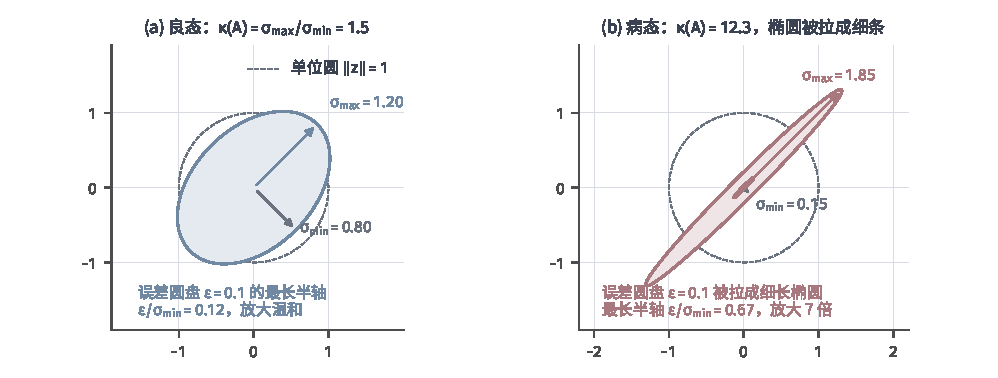
\includegraphics[width=169.0mm]{figures/00-shared/mathematical-preliminaries-upper/02-linear-spaces/matplotlib/ls-condition-number-amplification/ls-condition-number-amplification.pdf}
 \caption{条件数对误差圆盘的放大。灰虚线为单位圆$\lVert\bm z\rVert=1$；左为良态
 $\bm A_1=[[1,0.2],[0.2,1]]$，奇异值$1.20$与$0.80$，$\kappa_2=1.5$，像椭圆接近
 圆；右为病态$\bm A_2=[[1,0.85],[0.85,1]]$，奇异值$1.85$与$0.15$，$\kappa_2\approx12.3$，
 像被拉成细条。半径$\varepsilon=0.1$的误差圆盘（红）最长半轴为$\varepsilon/\sigma_{\min}$：
 良态为$0.125$，病态约$0.67$。}
 \label{fig:ls-condition-number-amplification}
\end{figure*}

条件数看的是方向之间的差异，不是矩阵元素或奇异值的大小。比较$\operatorname{diag}(1,s)$与$s\bm I$（$0<s<1$）：前者的奇异值为$1$与$s$，$\kappa_2=1/s$；后者的奇异值全为$s$，$\kappa_2=1$。$s\bm I$把每个向量都缩小，数值整体更小，但它对所有方向一视同仁：对任意$\bm x\neq\bm0$，$\kappa_{\mathrm{rel}}(s\bm I;\bm x)=s\lVert\bm x\rVert_2/(s\lVert\bm x\rVert_2)=1$，相对误差完全不被放大。$\operatorname{diag}(1,s)$只压缩第二个方向，示例~\ref{ex:ls-diagonal-relative-error-basepoints}中的放大正来自两个方向的这种差别。一般地，所有奇异值按同一比例缩放时条件数不变。

条件数也不描述反复作用的长期结果。下面两个矩阵的条件数相同，幂的变化趋势却相反。
\begin{example}[条件数相同而幂的趋势相反]
\label{ex:ls-condition-number-vs-powers}
给定同阶的$2\bm I$与$\tfrac12\bm I$。二者的奇异值分别全为$2$与全为$\tfrac12$，所以
\[
 \kappa_2(2\bm I)=\frac{2}{2}=1,\qquad
 \kappa_2\bigl(\tfrac12\bm I\bigr)=\frac{1/2}{1/2}=1 .
\]
但$(2\bm I)^k=2^k\bm I$逐次增长，$(\tfrac12\bm I)^k=2^{-k}\bm I$逐次衰减。
\end{example}
条件数衡量的是一次作用中相对误差的最坏放大，反复作用的长期行为要由谱半径判断（第~\ref{sec:ls-matrix-power-behavior}节），二者不能互相代替。

最后说明本节结论的适用范围。本节始终固定矩阵$\bm A$，只让输入向量带误差，条件数给出的是这种误差在一次线性作用中的最坏放大；它刻画问题本身的敏感性，不评价具体算法。第~\ref{sec:ls-numerical-sensitivity}节把输出改为方程的解，研究矩阵与右端同时带误差时的完整误差界，并区分数据误差与算法误差；第~\ref{sec:multivariable-inverse-differential}节再研究求逆和解映射对矩阵变化的一阶响应。下一节开始改变矩阵本身，分别检查特征值、奇异值和特征子空间。这些输出各有自己的敏感性度量，不能只凭$\kappa_2(\bm A)$判断它们是否敏感。
